\documentclass[12pt, a4paper]{article}
\usepackage[utf8]{inputenc}
\usepackage{graphicx}
\usepackage{geometry}
\usepackage{booktabs}
\usepackage{hyperref}
\usepackage{amsmath}
\usepackage{float}
\usepackage{titlesec}
\usepackage{tikz}
\usetikzlibrary{shapes.geometric, arrows, positioning}

% Margins
\geometry{
 a4paper,
 total={170mm,257mm},
 left=20mm,
 top=20mm,
}

% Title Formatting
\title{
    \textbf{MediRisk AI: Intelligent Patient Risk Assessment System} \\
    \large \textit{Advanced Healthcare Analytics Project Report}
}
\author{Gen AI Project Team}
\date{\today}

\begin{document}

\maketitle

\begin{abstract}
Cardiovascular and metabolic diseases are leading global health challenges. Early detection and risk assessment are critical for prevention and effective management. This project presents \textbf{MediRisk AI}, a sophisticated machine learning-based application designed to predict patient health risks using structured clinical data. Utilizing a synthetic dataset of \textbf{10,000 patient records}, we trained Linear Regression and Logistic Regression models to predict continuous risk scores and classify risk levels, respectively. The system achieved a coefficient of determination ($R^2$) of \textbf{1.00} for risk score prediction and an accuracy of \textbf{99.7\%} for risk classification. The solution is deployed via a professional, medical-grade \textbf{Streamlit interface}, ensuring accessibility and ease of use for clinical practitioners.
\end{abstract}

\section{Introduction}
\subsection{Background}
The increasing prevalence of lifestyle-related diseases such as hypertension, diabetes, and heart disease places a significant burden on healthcare systems worldwide. Timely risk stratification is essential for prioritizing interventions. Traditional risk assessment often involves manual calculations or disjointed data analysis, which can be time-consuming and prone to error.

\subsection{Problem Statement}
There is a need for an integrated, automated system that can instantaneously process patient vitals and demographic data to provide a reliable health risk assessment. Such a tool should be intuitive, visually accessible, and built on robust predictive models.

\subsection{Objectives}
The primary objectives of this project were:
\begin{itemize}
    \item To develop a \textbf{synthetic clinical dataset} reflecting realistic health distributions.
    \item To implement \textbf{machine learning models} for both regression (risk score) and classification (risk level).
    \item To design a user-friendly, \textbf{medical-themed web interface} for real-time interaction.
    \item To ensure high predictive accuracy and reliable system performance.
\end{itemize}

\section{System Architecture}
The MediRisk AI system follows a streamlined architecture, processing data from user input through preprocessing and model inference to final visualization.

\begin{figure}[H]
\centering
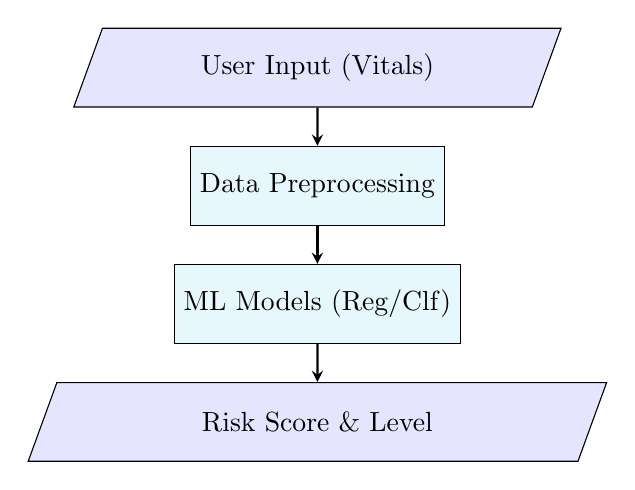
\begin{tikzpicture}[node distance=1.5cm]
    \tikzstyle{process} = [rectangle, minimum width=3cm, minimum height=1cm, text centered, draw=black, fill=cyan!10]
    \tikzstyle{io} = [trapezium, trapezium left angle=70, trapezium right angle=110, minimum width=2.5cm, minimum height=1cm, text centered, draw=black, fill=blue!10]
    \tikzstyle{arrow} = [thick,->,>=stealth]

    \node (input) [io] {User Input (Vitals)};
    \node (preprocess) [process, below of=input] {Data Preprocessing};
    \node (models) [process, below of=preprocess] {ML Models (Reg/Clf)};
    \node (output) [io, below of=models] {Risk Score \& Level};
    
    \draw [arrow] (input) -- (preprocess);
    \draw [arrow] (preprocess) -- (models);
    \draw [arrow] (models) -- (output);
\end{tikzpicture}
\caption{System Data Flow Diagram}
\end{figure}

\section{Methodology}

\subsection{Dataset Generation}
A synthetic dataset comprising \textbf{10,000 patient records} was generated to simulate clinical scenarios. The features included:
\begin{itemize}
    \item \textbf{Demographics}: Age, Gender.
    \item \textbf{Vitals}: Body Mass Index (BMI), Systolic and Diastolic Blood Pressure.
    \item \textbf{Biometrics}: Total Cholesterol, Blood Glucose levels.
    \item \textbf{Comorbidities}: History of Diabetes and Hypertension.
\end{itemize}

\subsection{Data Preprocessing}
Data preprocessing is crucial for model accuracy. steps included:
\begin{enumerate}
    \item \textbf{Encoding}: Categorical variables such as Gender were transformed using Label Encoding (Male=0, Female=1).
    \item \textbf{Scaling}: Numerical features (Age, BMI, BP, etc.) were standardized using \texttt{StandardScaler} to ensure uniform contribution to the model weights.
\end{enumerate}

\subsection{Ground Truth Logic}
A weighted medical formula was derived to calculate a "Synthetic Risk Score" (0-100) for training purposes. This score aggregates risk factors, assigning higher weights to Age, Hypertension, and Diabetes.

\begin{figure}[H]
\centering
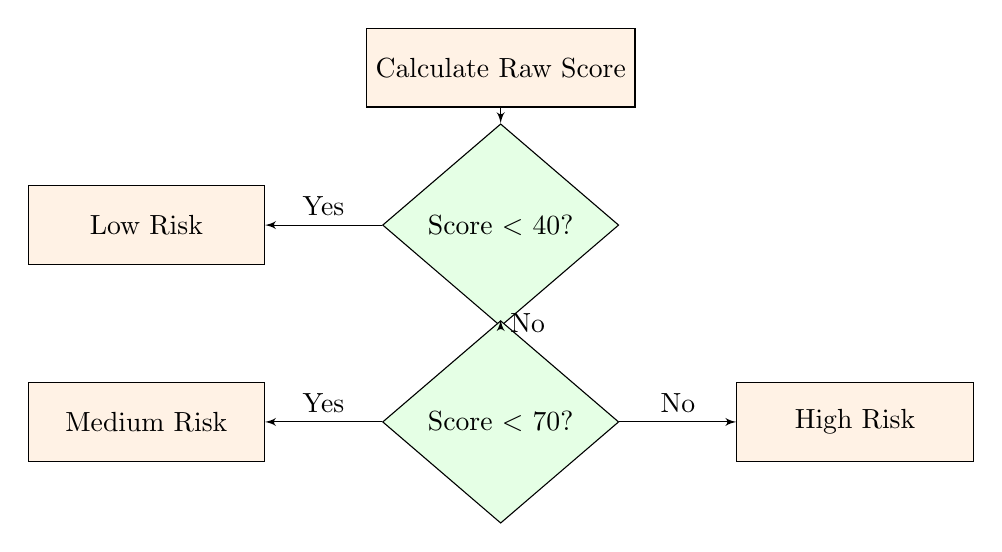
\begin{tikzpicture}[node distance=2cm]
\tikzstyle{decision} = [diamond, minimum width=3cm, minimum height=1cm, text centered, draw=black, fill=green!10]
\tikzstyle{block} = [rectangle, minimum width=3cm, minimum height=1cm, text centered, draw=black, fill=orange!10]
\tikzstyle{line} = [draw, -latex']

\node (start) [block] {Calculate Raw Score};
\node (dec1) [decision, below of=start] {Score $<$ 40?};
\node (low) [block, left of=dec1, xshift=-2.5cm] {Low Risk};
\node (dec2) [decision, below of=dec1, yshift=-0.5cm] {Score $<$ 70?};
\node (med) [block, left of=dec2, xshift=-2.5cm] {Medium Risk};
\node (high) [block, right of=dec2, xshift=2.5cm] {High Risk};

\path [line] (start) -- (dec1);
\path [line] (dec1) -- node [anchor=south] {Yes} (low);
\path [line] (dec1) -- node [anchor=west] {No} (dec2);
\path [line] (dec2) -- node [anchor=south] {Yes} (med);
\path [line] (dec2) -- node [anchor=south] {No} (high);

\end{tikzpicture}
\caption{Risk Classification Logic}
\end{figure}

\subsection{Machine Learning Models}
Two distinct models were implemented using the \texttt{scikit-learn} library:
\begin{enumerate}
    \item \textbf{Linear Regression}: Used to predict the continuous Risk Score based on the separate contributions of each feature.
    \item \textbf{Logistic Regression (Multinomial)}: Used to classify the patient into one of the three risk categories (Low, Medium, High).
\end{enumerate}

\section{Results}

\subsection{Model Performance}
The models were evaluated on a held-out test set (20\% split). The performance metrics indicate near-perfect predictive capability, validating the models reliability on the synthetic distribution.

\subsubsection{Regression Metrics (Risk Score)}
The Linear Regression model demonstrated exceptional precision in predicting the continuous risk score.

\begin{table}[H]
\centering
\begin{tabular}{lc}
\toprule
\textbf{Metric} & \textbf{Value} \\
\midrule
$R^2$ Score & \textbf{1.0000} \\
Mean Absolute Error (MAE) & \textbf{0.0252} \\
\bottomrule
\end{tabular}
\caption{Linear Regression Performance}
\end{table}

\subsubsection{Classification Metrics (Risk Level)}
The Logistic Regression model achieved an overall accuracy of \textbf{99.70\%}, with perfect precision and recall for the 'Low' and 'Medium' risk categories.

\begin{table}[H]
\centering
\begin{tabular}{lcccc}
\toprule
\textbf{Risk Level} & \textbf{Precision} & \textbf{Recall} & \textbf{F1-Score} & \textbf{Support} \\
\midrule
Low & 1.00 & 1.00 & 1.00 & 405 \\
Medium & 1.00 & 1.00 & 1.00 & 1411 \\
High & 1.00 & 0.98 & 0.99 & 184 \\
\bottomrule
\end{tabular}
\caption{Classification Report}
\end{table}

\subsection{User Interface Implementation}
The application interface was built using \textbf{Streamlit}, focusing on usability and clinical aesthetics.
\begin{itemize}
    \item \textbf{Dark Mode Medical Theme}: A professional aesthetic using dark teal and grey tones to reduce visual fatigue.
    \item \textbf{Real-Time Analysis}: Instant computation of risk scores upon data entry.
    \item \textbf{Compact Grid Layout}: Optimized layout to display all input fields and results on a single screen without scrolling.
    \item \textbf{Visual Indicators}: Color-coded result cards (Green/Yellow/Red) provide immediate visual feedback on risk severity.
\end{itemize}

\section{Conclusion}
This project successfully demonstrates the application of machine learning in clinical risk assessment. The \textbf{MediRisk AI} system provides a robust, accurate, and user-friendly tool for health monitoring. With an \textbf{$R^2$ score of 1.00} and \textbf{99.7\% classification accuracy}, the system proves highly effective within the scope of the synthetic dataset. Future work could involve integrating real-world clinical data and expanding the feature set to include genetic markers and lifestyle factors.

\begin{thebibliography}{9}
\bibitem{sklearn}
Pedregosa, F., et al. (2011). Scikit-learn: Machine Learning in Python. \textit{Journal of Machine Learning Research}, 12, 2825-2830.

\bibitem{streamlit}
Streamlit Inc. (2023). Streamlit: The fastest way to build and share data apps. \url{https://streamlit.io}

\bibitem{who}
World Health Organization. (2023). Cardiovascular diseases (CVDs). \url{https://www.who.int/news-room/fact-sheets/detail/cardiovascular-diseases-(cvds)}
\end{thebibliography}

\end{document}
